\documentclass[12p,a4paper]{report}
\usepackage[utf8]{inputenc}
\usepackage[T1]{fontenc,url}
\usepackage{multicol}
\usepackage{multirow}
\usepackage{parskip}
\usepackage{lmodern}
\usepackage{microtype}
\usepackage{verbatim}
\usepackage{amsmath, amssymb}
\usepackage{tikz}
\usepackage{physics}
\usepackage{mathtools}
\usepackage{algorithm}
\usepackage{algpseudocode}
\usepackage{listings}
\usepackage{enumerate}
\usepackage{graphicx}
\usepackage{booktabs}
\usepackage{float}
\usepackage{hyperref}
\usepackage{tabularx}
\usepackage{siunitx}
\usepackage{fancyvrb}
\usepackage{blindtext}
\usepackage{tcolorbox}
\usepackage{relsize}
\usepackage{wrapfig}
\usepackage[explicit]{titlesec} %Control margins around titles.
\usepackage[makeroom]{cancel}
\usepackage[margin=1.2cm]{geometry}
\renewcommand{\baselinestretch}{1}
\renewcommand{\exp}{e^}
\renewcommand{\b}{\boldsymbol}
\newcommand{\h}{\hat}
\newcommand{\m}{\mathbb}
\newcommand{\half}{\frac{1}{2}}
\renewcommand{\exp}{e^}
\renewcommand{\bar}{\overline}
\newcommand{\lRightarrow}{\mathlarger{\mathlarger{\Rightarrow}}}
\setlength\parindent{0pt}


% Colorcoding. First for inside equations, second for text.
\definecolor{lightyellow}{RGB}{255,255,80}
\definecolor{lightred}{RGB}{255,160,140}
\definecolor{lightgreen}{RGB}{180,255,180}
\definecolor{lightblue}{RGB}{180,220,255}
\definecolor{background_yellow}{RGB}{255,255,220}
\definecolor{background_red}{RGB}{255,180,150}
% Yellow
\newcommand{\yl}[1]{\colorbox{lightyellow}{$\displaystyle #1$}}
\newcommand{\yll}{\colorbox{lightyellow}}
% Green
\newcommand{\gr}[1]{\colorbox{lightgreen}{$\displaystyle #1$}}
\newcommand{\grr}{\colorbox{lightgreen}}
% Blue
\newcommand{\bl}[1]{\colorbox{lightblue}{$\displaystyle #1$}}
\newcommand{\bll}{\colorbox{lightblue}}
% Red
\newcommand{\rd}[1]{\colorbox{lightred}{$\displaystyle #1$}}
\newcommand{\rdd}{\colorbox{lightred}}


\renewcommand{\hat}{\widehat}


\usepackage{eqparbox}   
\titleformat{\chapter}[block]{}{\eqmakebox[chap]{\Large\MakeUppercase{\sffamily\lsstyle\chaptername} %
\raisebox{-0.6\height}{\fontsize{50pt}{50pt}\selectfont\thechapter}\quad}}{0pt}{\huge\bfseries\raisebox{1ex}{\parbox[t]{\dimexpr\textwidth-\eqboxwidth{chap}\relax}{\titlerule[2pt]\vspace{1.25ex}#1}}}
\titlespacing*{\chapter}{0pt}{-32pt}{48pt}













\begin{document}



%  ██████╗██╗  ██╗ █████╗ ██████╗ ████████╗███████╗██████╗     ██╗  ██╗
% ██╔════╝██║  ██║██╔══██╗██╔══██╗╚══██╔══╝██╔════╝██╔══██╗    ██║  ██║
% ██║     ███████║███████║██████╔╝   ██║   █████╗  ██████╔╝    ███████║
% ██║     ██╔══██║██╔══██║██╔═══╝    ██║   ██╔══╝  ██╔══██╗    ╚════██║
% ╚██████╗██║  ██║██║  ██║██║        ██║   ███████╗██║  ██║         ██║
%  ╚═════╝╚═╝  ╚═╝╚═╝  ╚═╝╚═╝        ╚═╝   ╚══════╝╚═╝  ╚═╝         ╚═╝
                                                                  
\setcounter{chapter}{3}
\chapter{Vector Spaces}
\section{Vector Spaces and the Invertible Matrix Theorem}
Let $A$ be an $m \times n$ matrix $A=[\b a_1, \dots , \b a_n]$

The \bll{\textbf{column space}} of $A$ is the span of its columns: \yll{$\text{Col}(A) = \text{Span}\{\b a_1, \dots , \b a_n\}$}. It's dimension is called the \textbf{rank} of $A$.

The \bll{\textbf{null space}} of $A$ is all vectors solving the equation \yll{$A \b x = \b 0$}.

The sum of their dimensions must equal the size of $A$: \grr{$\text{Dim}(\text{Col}(A)) + \text{Dim}(\text{Nul}(A)) = n$}.


$A$ will map any vector from $\m R^n$ onto some space $\m R^k$, where $k = \text{Rank}(A)$. The dimensions of the column space therefor decides the dimension of the space we map onto. The null space then represents all the dimensions that "disappear" during the transform.

\begin{tcolorbox}[title={The Invertible Matrix Theorem}]
\begin{itemize}
    \item $A$ is invertible.
    \item The columns of $A$ are linearly independent, and $A$ spans $\m R^n$.
    \item $A$ is row-equivalent to the identity matrix $I_n$.
    \item $A$ has $n$ pivot columns.
    \item The dimensions of $A$'s null space is zero. ($A\b x = \b x$ has only the solution $\b x = \b 0$).
    \item $0$ is not an eigenvalue of $A$.
    \item The determinant of $A$ is different from zero.
    \item $A^T$ is also invertible, and all of this applies to it.
\end{itemize}

\end{tcolorbox}



\section{Coordinate systems and mapping}
Consider a vector $\b x$ living in a vector space $V$. The vector $\b x$ is an abstract concept, living in some abstract space $V$. It may have some physical or gemoetric meaning or whatnot.

We now enforce a \textit{basis} onto $V$, called $\mathcal{B} = \{\b b_1,\dots, \b b_n\}$. This makes V \textit{behave like} $\m R^n$, in the sense that each vector $\b x$ in $V$ is \textit{mapped onto} a vector $[\b x]_\mathcal{B}$ in $\m R^n$. This is called a \textit{coordinate mapping} $\b x \mapsto [\b x]_\mathcal{B}$ "onto" the basis $\mathcal{B}$. The vector space $V$ might be foreign to us, and it can be important to create a mapping onto a more familiar vector space $\m R^n$, which we know how behaves. This transformation is \bll{"one-to-one"}, mapping each point in $V$ onto a point in $\m R^n$, and vice versa. This relation is called an \bll{\textbf{isomorphism}}, and makes any vector space $V$ with a basis of $n$ vectors \underline{indistinguishable from $\m R^n$}.

Usually, when a vector is written plainly as $\b x$, we consider it to be written in a \textit{standard basis} $\mathcal{E} = \{\b e_1,\, \b e_2\} = \begin{bmatrix} \,1\, \\ \,0\, \end{bmatrix},\, \begin{bmatrix} \,0\, \\ \,1\, \end{bmatrix}$, meaning that $\b x = [\b x]_\mathcal{E}$.

The relation between $\b x$ and $[\b x]_\mathcal{B}$ is given by a \textbf{change-of-basis matrix} $P_\mathcal{B}$, which consists of the basis-vectors of $\mathcal{B}$, written in the basis of $\mathcal{E}$:
\[
    \b x = P_\mathcal{B}[\b x]_\mathcal{B}  \quad\quad\quad  P_\mathcal{B} = [\b b_1\ \b b_2\ \dots\ \b b_n]
\]


\section{Change of basis}
This change of basis is just a special case of a more general change of basis between two basises $\mathcal{B} = \{\b b_1, \dots \b b_n\}$ and $\mathcal{C} = \{\b c_1, \dots \b c_n\}$, both spanning the same vector space $V$. The general change of basis is then
\[
    [\b x]_\mathcal{C} = \underset{\mathcal{C}\leftarrow\mathcal{B}}{P}\,[\b x]_\mathcal{B} \quad\quad\quad
    \underset{\mathcal{C}\leftarrow\mathcal{B}}{P} = \Big[[\b b_1]_\mathcal{C}\ [\b b_2]_\mathcal{C}\ \dots [\b b_1]_\mathcal{C}\Big]
\]

The change-of-basis matrix from $\mathcal{C}$ to $\mathcal{B}$ is simply the inverse: $\underset{\mathcal{B}\leftarrow\mathcal{C}}{P} = \qty(\underset{\mathcal{C}\leftarrow\mathcal{B}}{P})^{-1}$

The change of basis of a linear transformation is
\[
    [\,T\,]_\mathcal{C} = P\, [\,T\,]_\mathcal{B}\, P^{-1}
\]
where $P$ is the change-of-basis matrix $\underset{\mathcal{C}\leftarrow\mathcal{B}}{P}$

\section{Linear transformations (mappings) between vector spaces}

Any linear transformation is solely defined by how it acts on the unit vectors.

\begin{wrapfigure}{r}{10cm}
    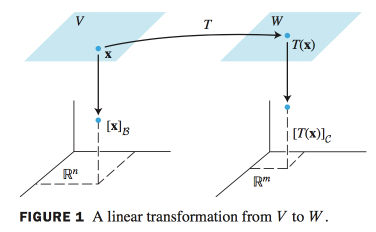
\includegraphics[width=8cm]{figs/map.jpg}
\end{wrapfigure} 
Consider two vector spaces $V$ and $W$, with basises $\mathcal{B} = \{\b b_1,\dots \b b_n\}$ and $\mathcal{C} = \{\b c_1,\dots, \b c_m\}$ in $\m R^n$ and $\m R^m$, respectively. We introduce a \textit{linear transformation} $T: V \mapsto W$ such that $T(\b x) = A\b x$. This is all well and good, but we might only have the vector $\b x$ represented in the basis $\mathcal{B}$, and usually want it written in the basis $\mathcal{C}$ after the transformation, as $\big[T(\b x)\big]_\mathcal{C}$.

What we want is some matrix $M$ that carries us straight from $[\b x]_\mathcal{B}$ to $\big[T(\b x)\big]_\mathcal{C}$. If we combine the change of basis with $T$, we get
\[
    \big[T(\b x)\big]_\mathcal{C} = M[\b x]_\mathcal{B}
\]
where
\[
    M = \Big[[T(\b b_1)]_\mathcal{C}\ \dots \ [T(\b b_n)]_\mathcal{C} \Big]
      = \Big[[A\b b_1]_\mathcal{C}\ \dots \ [A\b b_n]_\mathcal{C} \Big]
\]
This matrix is called the \textbf{matrix for T relative to the bases $\mathcal{B}$ and $\mathcal{C}$.}

If $M$ is invertible, there exists an inverse linear transform $T^{-1}$ with matrix representation $M^{-1}$, mapping every point in $\mathcal{B}$ to a point in $\mathcal{C}$. This makes $T$ an \textbf{isomorphism} (one-to-one mapping).





%  ██████╗██╗  ██╗ █████╗ ██████╗ ████████╗███████╗██████╗     ███████╗
% ██╔════╝██║  ██║██╔══██╗██╔══██╗╚══██╔══╝██╔════╝██╔══██╗    ██╔════╝
% ██║     ███████║███████║██████╔╝   ██║   █████╗  ██████╔╝    ███████╗
% ██║     ██╔══██║██╔══██║██╔═══╝    ██║   ██╔══╝  ██╔══██╗    ╚════██║
% ╚██████╗██║  ██║██║  ██║██║        ██║   ███████╗██║  ██║    ███████║
%  ╚═════╝╚═╝  ╚═╝╚═╝  ╚═╝╚═╝        ╚═╝   ╚══════╝╚═╝  ╚═╝    ╚══════╝
\chapter{Eigenvalues and Eigenvectors}
\section{Eigenvalues and Eigenvectors}
Let $A$ be an $n\times n$ matrix with eigenvalues $\lambda_1, \lambda_2,\dots, \lambda_n$ in decreasing order, and corresponding eigenvectors $\b v_1, \b v_2, \dots,\b v_n$.

\begin{itemize}
    \item The eigenvalues of $A$ is given by \textbf{the characteristic equation} \yll{$\text{Det}(A - \lambda I) = 0$}.
    \item If $A$ is \underline{triangular}, the eigenvalues are the entries of it's diagonal.
    \item If $A$ has \underline{$n$ distinct eigenvalues}, \bll{the eigenvectors are linearly independent}. If $A$ has degenerate eigenvalues, we have to check whether the eigenvector are independent or not.
\end{itemize}


\section{Diagonalization}
\begin{tcolorbox}[title={The Diagonalization Theorem}]
    An $n\times n$ matrix $A$ is diagonalizable if it has $n$ linearly independent eigenvectors.
\end{tcolorbox}

We can then write
\[
    A = P D P^{-1}
\]
where $D$ is a diagonal matrix and $P$ is an invertable matrix such that
\[
    D = \begin{pmatrix} \lambda_1 &           &         & \\
                                  & \lambda_2 &         & \\
                                  &           & \ddots  & \\
                                  &           &         & \lambda_n
        \end{pmatrix}
        \quad\quad
    P = \begin{pmatrix} \b v_1 & \b v_2 & \cdots & \b v_n \end{pmatrix}
\]

\section{Discrete dynamical systems}
Cosider a difference equation on the form
\[
    \b x_{i+1} = A\b x_i \quad\quad \Rightarrow \quad\quad \b x_k = A^k \b x_0
\]
where $\{\b x_0,\,\b x_1,\dots\}$ is a vector sequence describing the properties of some system, and $A$ is an $n\times x$ invertable matrix, giving it $n$ descrete eigenvalues, with $n$ orthogonal eigenvectors spanning $\m R^n$. This means any vector $x_i$ can be written as a linear combination of these:
\[
    x_i = c_1 \b v_1 + \dots + c_n \b v_n
\]
such that the matrix-vector multiplication $A^k \b x_0$ can be rewritten as
\[
    x_k = A^k x_0 = A^k\qty(c_1 \b v_1 + \dots + c_n \b v_n) = (\lambda_1)^k c_1 \b v_1 + \dots + (\lambda_n)^k c_n \b v_n
\]

In short, any such dynamical system can be decomposed into the eigenvectors of $A$, where the eigenvalues decides how the system behaves over time.

The coefficients are usually found as
\[
    \b c = P^{-1}\b x
\]

\subsection{Attractors}
We see that if all eigenvalues of $A$ are less than 1, the system will tend towards $\b 0$, and we say that $\b 0$ is an \textbf{attractor} for the system.


\section{Complex Eigenvalues}
Let $A$ be a real $2\times 2$ matrix with a complex eigenvalue $\lambda = a-bi$, and an associated eigenvector $\b v$. Then
\[
    A = PCP^{-1}, \quad \text{where} \quad P = \big[\, \text{Re}(\b v) \ \text{Im}(\b v)\, \big] \quad \text{and} \quad C = \begin{pmatrix} a & -b \\ b & a \end{pmatrix}
\]


\section{Applications to Differential Equations}
Consider the system of equations
\begin{align*}
    x_1' &= a_{11}x_1 + \dots + a_{1n}x_n \\
    x_2' &= a_{21}x_1 + \dots + a_{2n}x_n \\
    &\vdots \\
    x_n' &= a_{n1}x_1 + \dots + a_{nn}x_n
\end{align*}
where $x_i$ are differentiable functions of $t$.

This problem can be written as the matrix problem
\[
    \b x'(t) = A\b x(t)
\]
where we need to solve it for some known $t$.

%  ██████╗██╗  ██╗ █████╗ ██████╗ ████████╗███████╗██████╗      ██████╗ 
% ██╔════╝██║  ██║██╔══██╗██╔══██╗╚══██╔══╝██╔════╝██╔══██╗    ██╔════╝ 
% ██║     ███████║███████║██████╔╝   ██║   █████╗  ██████╔╝    ███████╗ 
% ██║     ██╔══██║██╔══██║██╔═══╝    ██║   ██╔══╝  ██╔══██╗    ██╔═══██╗
% ╚██████╗██║  ██║██║  ██║██║        ██║   ███████╗██║  ██║    ╚██████╔╝
%  ╚═════╝╚═╝  ╚═╝╚═╝  ╚═╝╚═╝        ╚═╝   ╚══════╝╚═╝  ╚═╝     ╚═════╝
\chapter{Orthogonality and least squares}
\section{Orthogonal Matrixes}
Consider an $m\times n$ matrix $U$ with \bll{orthonormal columns}. We call this an orthonormal matrix. This matrix has the properties:
\begin{itemize}
    \item $U$ is orthonormal only if $U^T U = I$.
    \item $U$ preserves length: $||U \b x|| = ||\b x||$.
    \item If $U$ is square, we have that \yll{$U^{-1} = U^T$}.
\end{itemize}


\section{Projections}
\subsection{Projection of vector onto vector}
The projection of a vector $\b y$ onto another vector $\b x$ is
\begin{align*}
    \hat{\b y} = \yl{\text{proj}_{\b x}(\b y) = \frac{\b y \cdot \b x}{\b x \cdot \b x}\b x}
\end{align*}



\subsection{Projection of vector onto subspace}
Let $W$ be subspace of $\m R^n$ with an orthogonal basis $\{\b u_1, \dots, \b u_p\}$ and $\b y$ be any vector in $\m R^n$. Then the projection of $\b y$ onto $W$ is simply the projection onto each basis-vector:
\begin{align*}
    \hat{\b y} = \yl{\text{proj}_{W}(\b y) =\frac{\b y \cdot \b u_1}{\b u_1 \cdot \b u_1}\b u_1 + \dots + \frac{\b y \cdot \b u_p}{\b u_p \cdot \b u_p}\b u_p}
\end{align*}
If you have an \underline{orthonormal} basis, the dot products reduces to $1$, and this can be written.
\begin{align*}
    \hat{\b y} = \yl{\text{proj}_{W}(\b y) = (\b y\cdot \b u_1)\b u_1 + \dots + (\b y\cdot \b u_n)\b u_n = U U^T \b y}
\end{align*}
where $U = [\b u_1,\dots \b u_n]$ contains the basis vectors.



\section{The Gram-Schmidt process of orthogonal factorization}
The Gram-Schmidt process takes any basis of vectors $\{\b x_1, \dots, \b x_p\}$ spanning a subspace in $\m R^n$, and creates a new \textit{orthogonal} basis of the same space, $\{\b v_1, \dots, \b v_p\}$.

The idea is to create one and one new vector $\b v_i$ from the corresponding $\b x_i$, \textit{but} subtract the projection of $\b x_i$ onto each of the former vectors $\b v_1, \dots, \b v_{i-1}$, such that the new vector is orthogonal to all formerly created vectors.
\begin{itemize}
    \item $\b v_1 = \b x_1$
    \item $\b v_2 = \b x_2 - \dfrac{\b x_2 \cdot \b v_1}{\b v_1 \cdot \b v_1}\b v_1$
    \item $\b v_3 = \b x_3 - \dfrac{\b x_3 \cdot \b v_1}{\b v_1 \cdot \b v_1}\b v_1
     - \dfrac{\b x_3 \cdot \b v_2}{\b v_2 \cdot \b v_2}\b v_2$
    \item \dots
\end{itemize}
Remember to normalize afterwards if you need an \textit{orthonormal} basis.


\section{QR-factorization}
If the columns of any $m\times n$ matrix $A$ are linearly independent, it can be QR-factorized:
\begin{tcolorbox}
    \grr{$A = QR$}
    \begin{itemize}
        \item \yll{$Q = [\b u_1 \ \b u_2 ... \b u_n]$} where $\b u_i$ is an \underline{orthonormal} basis for the columnspace of $A$. Simply use Gram-Schmidt on the columns of $A$, and normalize them.
        \item \yll{$R = Q^{-1}A = Q^T A$}, because $Q^T = Q^{-1}$ due to orthonormal columns. $R$ will always be upper diagonal.
    \end{itemize}
\end{tcolorbox}


\section{Least-sqaure problems}
Let $W$ be the column space of some matrix $A$: $W = \text{span}\{\text{col}(A)\}$.

Sometimes, the equation $A\b x = \b b$ has no solutions, because $\b b$ is not in $W$. We then often wish to find the solutions $\hat{\b x}$ which places the solutions $A\hat{\b x} = \hat{\b b}$ as close to the actual solution $\b b$ as possible.

This "closest solution" is the projection of $\b b$ onto $W$, $\hat{\b b} = \text{proj}_{W} \b b$.

The \bll{least-square solution} to \grr{$A\b x = \b b$} is then:
\begin{align*}
    \yl{A\hat{\b x} = \hat{\b b}} \quad \Rightarrow\quad
    \yl{\hat{\b x} = A^{-1}\hat{\b b}} \quad\quad(=A^{-1}AA^T\b b)
\end{align*}


If we have a $QR$ factorization of $A$, we can solve the least square problem as
\[
    \hat{x} = R^{-1}Q^T \b b
\]


\subsection{Applications to linear models}
Let's say we wish to fit some data $(x_1, y_1), (x_2, y_2),\dots$ to a linear model $y(x) = \beta_0 + \beta_1 x$.
\begin{figure}[H]
    \includegraphics[width=0.7\textwidth, trim={0cm 8cm 0cm 9cm}]{figs/fig.pdf}
\end{figure}
which produces a least-square solution $X\hat{\beta} = \hat{y}$.

%  ██████╗██╗  ██╗ █████╗ ██████╗ ████████╗███████╗██████╗     ███████╗
% ██╔════╝██║  ██║██╔══██╗██╔══██╗╚══██╔══╝██╔════╝██╔══██╗    ╚════██║
% ██║     ███████║███████║██████╔╝   ██║   █████╗  ██████╔╝        ██╔╝
% ██║     ██╔══██║██╔══██║██╔═══╝    ██║   ██╔══╝  ██╔══██╗       ██╔╝ 
% ╚██████╗██║  ██║██║  ██║██║        ██║   ███████╗██║  ██║       ██║  
%  ╚═════╝╚═╝  ╚═╝╚═╝  ╚═╝╚═╝        ╚═╝   ╚══════╝╚═╝  ╚═╝       ╚═╝
\chapter{Symmetric Matrices and Quadratic Forms}

\section{Diagonalization of symmetric Matrices}
A \bll{symetric} matrix $A$ is such that $A^T = A$.

If $A$ is symetric, any two eigenvectors from different eigenspaces are \underline{orthogonal}.

A is then \bll{orthogonally diagonalizable}, such that $A = PDP^{-1} = PDP^T$, where $P$ consists of $A$'s orthogonal eigenvectors.

\section{Quadratic Forms}
Consider a function \bll{$Q: \m R^n \mapsto \m R$} given by \grr{$Q(\b x) = \b x^T A \b x$} called a \yll{\textbf{quadratic form}}, defined by a \underline{symmetric} $n\times n$ matrix $A$.\\
The result will then be a second order polynomial
\[
    c_{00}\, x_1^2 + c_{11}\, x_2^2 + c_{12}\, x_1 x_2 + ...
\]
The matrix will then be a form
\[
    A = \begin{pmatrix}
        c_{00} & \half c_{12} & \half c_{13} & \cdots \\
        \half c_{12} & c_{11} & & \\
        \vdots & & \ddots & \\
        & & & c_{nn}
    \end{pmatrix}
\]
The non-diagonals are halved, because they "share" the coefficients due to the symetry.

\begin{tcolorbox}
    If the eigenvalues of $A$ are 
    \begin{itemize}
        \item All positive, $Q(\b x)$ takes only positive values in $\m R$.
        \item All negative, $Q(\b x)$ takes only negative values in $\m R$.
    \end{itemize}
\end{tcolorbox}

\subsection{Change of variable}
Let $A = PDP^{-1}$. We can then substitute $\b x = P \b y$, giving
\[
    \b xx^T A \b x = \b y^t D y
\]
where $D$ is diagonal.


\section{Constraint optimization}
We often wish to solve for the $\b x$ that gives the maximum or minimum $Q(\b x)$ under some constraint $||\b x || = ||\b x^2|| = \b x^T \b x = 1$.

\begin{itemize}
    \item The maximum value of $Q(\b x)$ is the largest eigenvalue of $A$. The $\b x$ giving this value is the corresponding eigenvector.
    \item The minimum value of $Q(\b x)$ it the smallest eigenvalue of $A$. The $\b x$ giving this value is the corresponding eigenvector.
\end{itemize}



\section{Singular Value Decomposition}
We know the $A = PDP^{-1}$ diagonalization of $A$ can only be applied to $n\times n$, diagonalizable matrices $A$.

However, the \yll{\textbf{singular value decomposition}} \bll{$A = U\Sigma V$} can be applied to \textit{any} matrix $A$. It reduces to $PDP^{-1}$ factorization if $A$ is diagonalizable.

\begin{tcolorbox}
    \begin{itemize}
    \item The \yll{singular values} of $A$ are the squareroots of the eigenvalues of $A^T A$, in decreasing order:
    \[
        \gr{\sigma_i = \sqrt{\lambda_i}}
    \]

    \item The \yll{singular vectors} of $A$ are the \underline{normalized} eigenvectors of $A^T A$, ordered by decending eigenvalues.
    \end{itemize}
\end{tcolorbox}


\begin{tcolorbox}
    Let $A$ be some $m\times n$ matrix with rank $r$. Then $A$ can be factorized into $A = U\Sigma V$ where \\
    \begin{itemize}
        \item $\Sigma$ is a $m\times n$ matrix (same shape as $A$), where the diagonal values are all the \underline{singular values} of $A$, with trailing zeros.
            \[ \Sigma = 
            \begin{pmatrix}
                \sigma_1 & 0 & 0 & 0 & 0 \\
                0 & \sigma_2 & 0 & 0 & 0 \\
                0 & 0 & \sigma_3 & 0 & 0 \\
                0 & 0 & 0 & 0 & 0
            \end{pmatrix}
            \]

        \item $V$ is an orthogonal $n\times n$ matrix, consisting of the \underline{singular vectors} of $A$:
            \[
                V = 
                \begin{pmatrix}
                    \b v_1 & \b v_2 & \b v_3
                \end{pmatrix}
            \]

        \item $U$ is an orthogonal $m\times m$ matrix where the columns are the normalized $A v_i$ vectors:
            \[  U = 
                \begin{pmatrix}
                    \dfrac{A \b v_1}{\sigma_1} & \dfrac{A \b v_2}{\sigma_2} & \dfrac{A \b v_3}{\sigma_3}
                \end{pmatrix}
            \]
            If there aren't $m$ non-zero vectors to use, construct the rest of $U$ as orthonormal vectors from Gram-Schmidt.
    \end{itemize}
\end{tcolorbox}



\chapter{Matlab}
\subsection*{Poly(A)}
Returns the negative of the characteristic polynomial of $A$.\\
Ex:
\begin{align*}
    \text{INPUT:} \quad \text{poly}(A) \\
    \text{OUTPUT:} \quad 1\ {-4}\ 3\ 0 \\
    \Rightarrow \ -(\lambda^3 - 4\lambda^2 + 3\lambda + 0) = 0
\end{align*}


\end{document}
